\section{YAG reakcijos matematinis modeliavimas}

Šiame darbe yra modeliuojama kietafazė reakcija, kurios metu reaguodami itrio ir aliuminio oksidai sudaro itrio aliuminio granato kristalus arba tiesiog \acs{yag}:
\begin{align*}
  \ce{3Y_2O_3 + 5Al_2O_3 -> 2Y_3Al_5O_12}
\end{align*}

Prieš pradedant reakciją metalų oksidai yra sutrinami iki smulkiagrūdžių miltelių ir maišomi kol susidaro homogeniškas mišinys. Metalų oksidų mišinys yra nuolat kaitinamas 1600\degree C laipsnių temperatūroje ir periodiškai maišomas. Eksperimentiniu būdu išmatuota, kad individualių mikrodalelių turiai prie 1600\degree C temperatūros siekia apie $10\mu\text{m}^3$ \cite{ivanauskasComputationalModellingYAG2009}. Tokioje temperatūroje metalų oksidai lydosi ir vyksta medžiagų difuzija, todėl reakcijos produktas formuojasi ties mikrodalelių sienelėmis.

\begin{figure}[h]
  \centering
  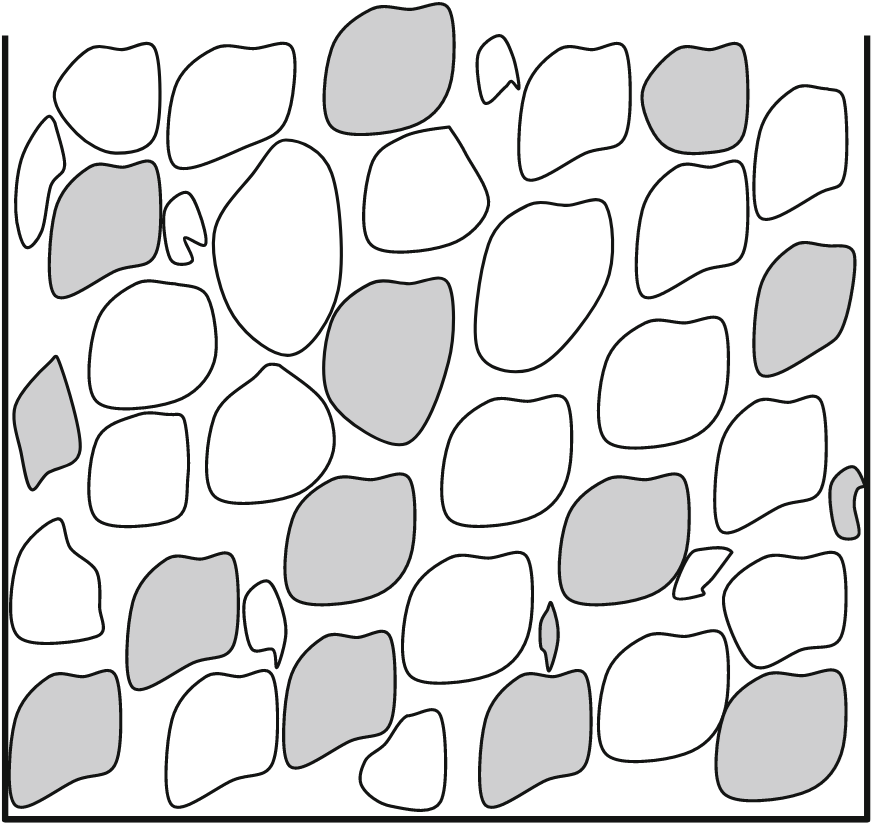
\includegraphics[width=0.25\linewidth]{assets/metal_oxides_mixture.png}
  \caption{Priartinto metalų oksidų mišinio iliustracija}
  \label{fig:metal-oxides-mixuter}
\end{figure}

Verta paminėti, kad \ref{fig:metal-oxides-mixuter}-ame pavyzdyje matoma iliustracija nėra iki galo tiksli, yra žinoma, kad mikrodalelės yra išsidėsčiusios glaudžiai.
\cite{ivanauskasModellingSolidState2005} Ivanauskas et al pasiūlė modelį, kuriame mikrodalelės yra laikomos kubo arba kvadrato formos priklausomai nuo dimensijos, kurioje modeliuojama reakciją. Laikoma, kad dalelės erdvėje yra periodiškai pasikartojančios, todėl užtenka modeliuoti mažą sritį, kurioje susiduria skirtingų medžiagų dalelės. 

\begin{figure}[h]
  \centering
  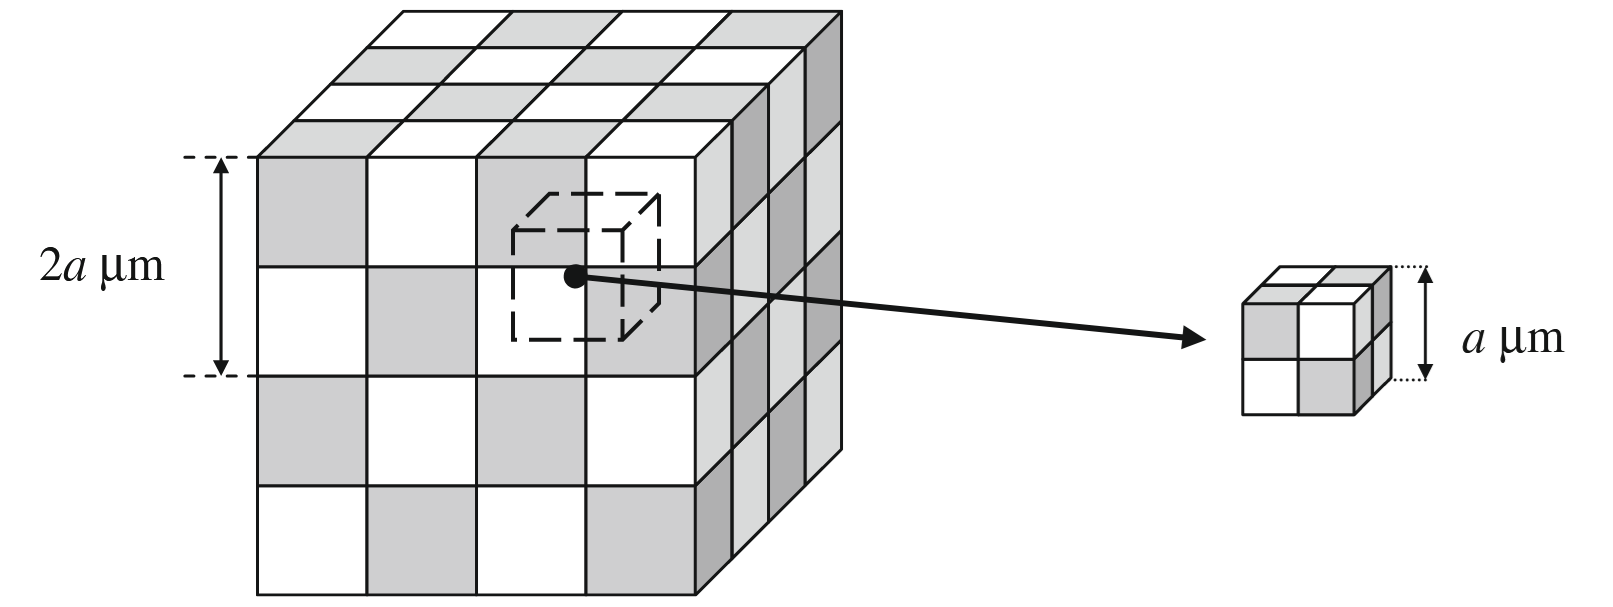
\includegraphics[width=0.75\linewidth]{assets/periodic-space.png}
  \caption{Periodiškas reakcijos erdvės modelis, čia dalelės tūris $V=a^3=10\mu m$}
  \label{fig:periodic-space}
\end{figure}

Vykstant reakcijai, chemikai periodiškai ištraukia reagentus iš krosnies, kurioje vyksta reakcija, todėl maišymas vyksta prie daug žemesnės temperatūros. Milteliai yra išmaišomi nepažeidžiant mikrodalelių struktūros - t. y. maišoma taip, kad mikrodalelės neskiltų.